\documentclass[border=10pt]{standalone}
\usepackage[utf8]{inputenc}
\usepackage{tikz}
\usepackage{pgfplots}
\pgfplotsset{compat=1.18}
\usepackage{xcolor}

\definecolor{cBlue}{HTML}{2C3E50}
\definecolor{cBrown}{HTML}{8B4513}
\definecolor{cGray}{HTML}{7F8C8D}
\definecolor{cGreen}{HTML}{27AE60}
\definecolor{cRed}{HTML}{C0392B}

\pgfplotsset{
  tbtf base/.style={
    width=12cm,
    grid=major,
    grid style={gray!20},
    tick label style={font=\small},
    label style={font=\small},
  }
}

\begin{document}
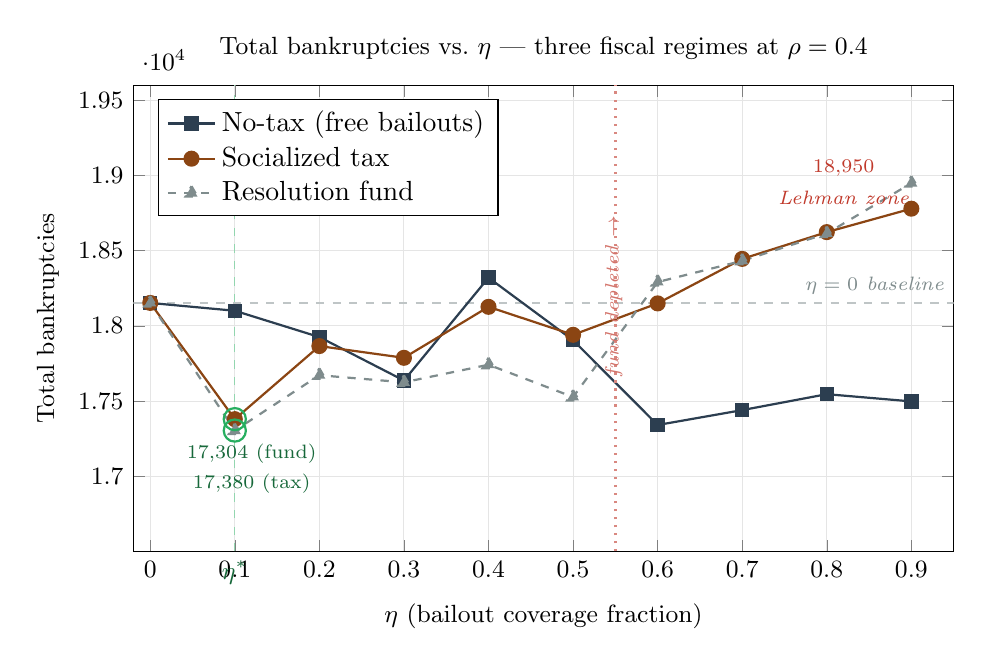
\begin{tikzpicture}
\begin{axis}[
  tbtf base,
  height=7.5cm,
  xlabel={$\eta$ (bailout coverage fraction)},
  ylabel={Total bankruptcies},
  xtick={0,0.1,0.2,0.3,0.4,0.5,0.6,0.7,0.8,0.9},
  xmin=-0.02, xmax=0.95,
  ymin=16500, ymax=19600,
  ytick={17000,17500,18000,18500,19000,19500},
  title={\small Total bankruptcies vs.\ $\eta$ --- three fiscal regimes at $\rho=0.4$},
  legend pos=north west,
  legend cell align=left,
  extra x ticks={0.1},
  extra x tick labels={$\eta^*$},
  extra x tick style={grid=major, grid style={dashed, cGreen!50},
                      tick label style={color=cGreen!60!black, font=\small}},
]

\draw[dashed, color=cGray!50, line width=0.6pt]
  (axis cs:-0.02,18153) -- (axis cs:0.95,18153);
\node[font=\scriptsize\itshape, color=cGray, anchor=east] at (axis cs:0.95,18270)
  {$\eta=0$ baseline};

\addplot[color=cBlue, mark=square*, mark size=2.2pt, thick]
  coordinates {
    (0,18153)(0.1,18101)(0.2,17926)(0.3,17637)(0.4,18321)
    (0.5,17905)(0.6,17341)(0.7,17440)(0.8,17546)(0.9,17498)
  };
\addlegendentry{No-tax (free bailouts)}

\addplot[color=cBrown, mark=*, mark size=2.5pt, thick]
  coordinates {
    (0,18153)(0.1,17380)(0.2,17866)(0.3,17788)(0.4,18127)
    (0.5,17941)(0.6,18150)(0.7,18446)(0.8,18624)(0.9,18780)
  };
\addlegendentry{Socialized tax}

\addplot[color=cGray, mark=triangle*, mark size=2.5pt, thick, dashed]
  coordinates {
    (0,18153)(0.1,17304)(0.2,17672)(0.3,17625)(0.4,17742)
    (0.5,17527)(0.6,18292)(0.7,18433)(0.8,18615)(0.9,18950)
  };
\addlegendentry{Resolution fund}

\addplot[color=cGreen, mark=o, mark size=4pt, only marks, thick, forget plot]
  coordinates {(0.1,17380)(0.1,17304)};

\draw[dotted, color=cRed!60, line width=0.9pt]
  (axis cs:0.55,16500) -- (axis cs:0.55,19600);
\node[font=\scriptsize\itshape, color=cRed!70, rotate=90, anchor=south]
  at (axis cs:0.57,18200) {fund depleted $\rightarrow$};

\node[font=\scriptsize, color=cRed] at (axis cs:0.82,19050)
  {18,950};
\node[font=\scriptsize\itshape, color=cRed] at (axis cs:0.82,18850)
  {Lehman zone};

\node[font=\scriptsize, color=cGreen!60!black] at (axis cs:0.12,17150)
  {17,304 (fund)};
\node[font=\scriptsize, color=cGreen!60!black] at (axis cs:0.12,16950)
  {17,380 (tax)};

\end{axis}
\end{tikzpicture}
\end{document}
